\pagebreak
\section{Anhang}
\subsection{Speicherung der Daten einer Veröffentlichung -
            \glqq Dummy-Paper\grqq{}}\label{app:dummy-paper}
\begin{wrapfigure}{r}{0.5\linewidth}
  \vspace{-1em}
  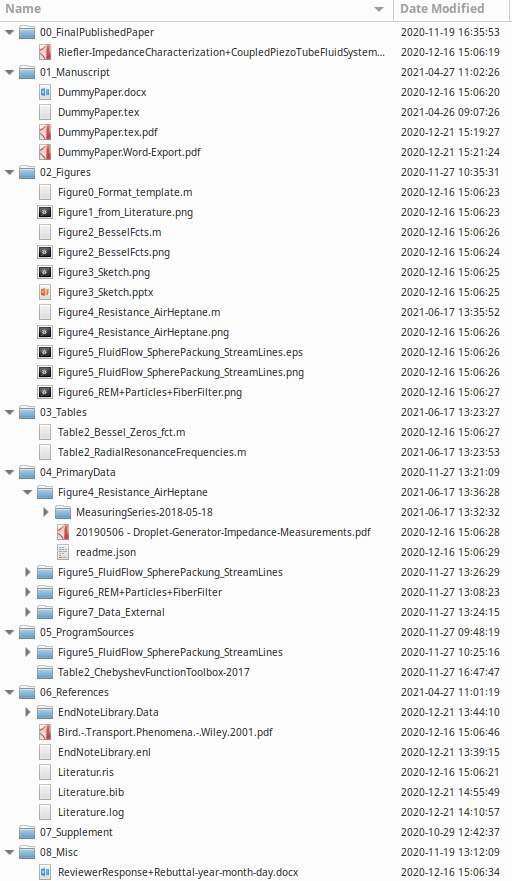
\includegraphics[width=\linewidth]{Figure03_DummyPaperStructureExample4.png}
  \caption{Complete data structure of a dummy paper.}
  \label{fig:dummy-paper}
\end{wrapfigure}
Der folgende Screenshot zeigt die komplette Datenstruktur eines Dummy-Papers.
Sie finden dieses Dummy Paper auf unserem VT-Server
\href{http://gofile.me/6C5nG/0uMzVrlwb}{hier}
(\url{http://gofile.me/6C5nG/0uMzVrlwb}),
zusammen mit diesen Richtlinien. Grundsätzlich geht es darum, dass alle Daten im
Paper, egal ob es sich um eine Abbildung oder eine Tabelle handelt, mit der
ursprünglichen Quelle der Messung oder der Simulation in Verbindung gebracht
werden können. Dies wird im Dummy Paper durch Matlab-Skripte realisiert, kann
aber auch mittels Python oder Excel erfolgen. Entscheidend ist: Egal wie, aber
es muss ein Bezug zwischen den im Verzeichnis \texttt{'04\_PrimaryData'}
gespeicherten Daten und ihrer Darstellung in der Publikation hergestellt werden. Alle
Abbildungen und die dazugehörigen Skripte - hier Matlab-Dateien - werden
zusammen mit den Messdaten angegeben, so dass die Ausführung eines
Matlab-Skripts in diesem Verzeichnis die entsprechende Abbildung erzeugt, damit
schließlich Ihre Ergebnisse in Ihrer Veröffentlichung nachvollzogen werden
können. Im Falle von anderen Daten, wie z.B. REM-Bildern, können Sie auf diese
durch ein vom ELN generiertes PDF verweisen, das einen Link zu dem dort
gespeicherten Experiment enthält.

Das "Dummy Paper" \verb+e+nthält eine Word- und eine LaTeX-Vorlage in
\texttt{'01\_Manuscript'}. Die EndNote- oder BibTeX-Literaturreferenzen
befinden sich in \texttt{'06\_References'}. Beide, die EndNote-Datei '*.enl'
oder die BibTeX-Datei '*.bib', sollten Links zwischen den Referenzen und den
frei zugänglichen PDFs der Papiere und Bücher enthalten, die ebenfalls in
\texttt{'06\_References'} gespeichert sind.

\subsection{Schreiben eines Datenmanagementplans}

\subsubsection{Motivation}

Ein Datenmanagementplan (DMP) dokumentiert die Überlegungen eines Antragstellers
zu den Daten, die im Rahmen eines laufenden Forschungsprojekts anfallen.
Forschungsförderer (DFG etc.) erwarten mittlerweile, dass öffentlich geförderte
Projekte ihre Daten der Öffentlichkeit zugänglich machen, wofür in der
Vergangenheit eine einfache Veröffentlichung ausreichte.

Aufgrund der Vielzahl unterschiedlicher Forschungsaufgaben gibt es keine
einheitliche Struktur für DMPs. Im Folgenden sind die wesentlichen Elemente
eines DMP der TIB Hannover aufgeführt, die sich so auch bei den Empfehlungen der
DFG wiederfinden.\\
(\url{https://www.dfg.de/download/pdf/foerderung/grundlagen_dfg_foerderung/forschungsdaten/forschungsdaten_checkliste_de.pdf})

\subsubsection{Elemente eines DMP}

\begin{enumerate}[start=0, label=\textbf{\arabic*})]
  \item \textbf{Administrative Informationen}
        \begin{itemize}
          \item Projektname
          \item Projektteilnehmende
          \item Projektbeschreibung
          \item Projektgrund (Promotion, Drittmitel, etc.)
          \item Projektdauer
          \item Version des DMP
        \end{itemize}
  \item \textbf{Methoden und Arten der Datenerhebung}
        \begin{itemize}
          \item Werden Primärdaten generiert oder werden Sekundärdaten verwendet?
        \item Welche Datentypen/-formate werden erzeugt und verarbeitet?
        \item Wie groß sind die Daten?
        \item Welche Ausrüstung (Instrumente, Hardware, Software usw.) wird
              verwendet?
        \item Wie sind die Daten organisiert? (Verzeichnis oder dateiorientierte
              Struktur? Versionskontrolle?)
        \item Wie werden der Forschungsprozess und die Daten dokumentiert?
        \item Welche (technischen) Standards werden für die
              Beschreibung/Dokumentation verwendet (Metadaten, Klassifizierung)?
        \item Wie werden die Metadaten erzeugt (z.B. automatisch, manuell, nach
              einem Leitfaden, selbst definiert)?
        \end{itemize}
  \item \textbf{Sicherung und Datensicherheit}
        \begin{itemize}
          \item Wo werden die Daten gespeichert?
          \item Welche Kapazität wird benötigt?
          \item Intervall der Datensicherheit?
          \item Sind irgendwelche Schutzmaßnahmen für sensible Daten erforderlich?
          \item Gibt es Dritte unter den Projektpartnern (z. B. bei gemeinsamen
                Projekten), die Zugang zu den Daten benötigen?
        \end{itemize}
  \item \textbf{Archivierung}
        \begin{itemize}
          \item Welche Daten werden archiviert?
          \item Auf welchem Datenträger?
          \item Gibt es Anforderungen an die Betreiberinnen und Betreiber der Infrastruktur? Z.B.
                Datenkuratierung?
          \item Welche Metadaten müssen bereitgestellt werden, um die
                archivierten Daten zu finden?
          \item Welche Informationen werden zusätzlich benötigt, um den
                Kontext der Daten zu verstehen?
          \item Wie lange werden die Daten archiviert?
          \item Gibt es rechtliche Besonderheiten bei der Datenarchivierung?
          \item Wie hoch sind die Kosten für welche Dienstleistung?
        \end{itemize}
  \item \textbf{Gemeinsame Nutzung und Veröffentlichung von Daten}
        \begin{itemize}
          \item Gibt es Daten, die mit anderen geteilt werden müssen?
          \item Welche Systeme sind für die gemeinsame Nutzung der Daten möglich?
          \item Welche Metadaten und Dokumentationen werden zusätzlich benötigt,
                damit Dritte die Daten nutzen können?
          \item Wo (Datenrepositorium, Datenzeitschrift) werden die Daten
                veröffentlicht und wie (z.B. Open Access, mit Sperrfrist,
                beschränkter Zugang)?
          \item Wie lauten die Lizenzbedingungen für die veröffentlichten Daten?
               (z. B. "CC BY 4.0")
        \end{itemize}
  \item \textbf{Ressourcen und Verantwortlichkeiten}
        \begin{itemize}
          \item Wie ist die Verteilung der Verantwortung in diesem Projekt
                geregelt?
          \item Wer ist für das Datenmanagement verantwortlich (Prozesse, IT,
                Richtlinien, Formate, Monitoring)?
          \item Erforderliche personelle Ressourcen für eine erfolgreiche
                Implementierung/Realisierung?
          \item Wie hoch sind die Kosten innerhalb der Projektphase und ggf.
                danach?
          \item Welche Infrastruktur-Ressourcen werden benötigt, fallen
                zusätzlichen Kosten an?
        \end{itemize}
\end{enumerate}
